%% LyX 2.1.3 created this file.  For more info, see http://www.lyx.org/.
%% Do not edit unless you really know what you are doing.
%% This specific layout has been created by:
%% Antonio Fernández Ares
%% antares@ugr.es
%% Github @deantares
\documentclass[a4paper,spanish]{scrartcl}
\usepackage[T1]{fontenc}
\usepackage[utf8]{inputenc}
\usepackage{fancyhdr}
\pagestyle{fancy}
\usepackage{color}
\definecolor{note_fontcolor}{rgb}{1, 0.335938, 0}
\usepackage{array}
\usepackage{float}
\usepackage{endnotes}
\usepackage{graphicx}
\usepackage{setspace}
\onehalfspacing

\makeatletter

%%%%%%%%%%%%%%%%%%%%%%%%%%%%%% LyX specific LaTeX commands.
\pdfpageheight\paperheight
\pdfpagewidth\paperwidth

%% Because html converters don't know tabularnewline
\providecommand{\tabularnewline}{\\}
%% The greyedout annotation environment
\newenvironment{lyxgreyedout}
  {\textcolor{note_fontcolor}\bgroup\ignorespaces}
  {\ignorespacesafterend\egroup}

%%%%%%%%%%%%%%%%%%%%%%%%%%%%%% Textclass specific LaTeX commands.
 \let\footnote=\endnote

%%%%%%%%%%%%%%%%%%%%%%%%%%%%%% User specified LaTeX commands.
\usepackage{colortbl}

\definecolor{azulclaro}{rgb}{0.6,0.8,1}

%Aumentar el padding de las tablas
\usepackage{array}
\setlength\extrarowheight{3pt}

%Usar paquete xymatrix
\usepackage[all]{xy}


%Usar paquete para resaltado de código :)
\usepackage{listings}

%Usar paquete para gráficos
\usepackage{tikz}

\usepackage{pgfgantt}

%\newcommand{\paquete}[1]{\[\texttt{#1} \]}

\makeatother

\usepackage{babel}
\addto\shorthandsspanish{\spanishdeactivate{~<>}}

\begin{document}

\lhead{
\includegraphics[height=1cm]{imgs/ugrLogo}}


\rhead{
\includegraphics[height=1cm]{imgs/posgradoLogo!}}


\title{Plan Investigación}


\author{Paloma de las Cuevas Delgado}


\subtitle{
\includegraphics[height=2cm]{imgs/ugrLogo}}

\maketitle
\newpage{}

\begin{center}
\begin{table}[H]
\centering{}%
\begin{tabular}{>{\raggedleft}m{5cm}>{\raggedright}m{8cm}}
\hline 
\multicolumn{2}{|c|}{\textcolor{cyan}{\cellcolor{azulclaro}}Plan de Investigación}\tabularnewline
\hline 
\hline 
\multicolumn{2}{|l|}{\textcolor{cyan}{\cellcolor{azulclaro}} Doctorando:}\tabularnewline
\hline 
Apellidos y nombre: & de las Cuevas Delgado, Paloma \tabularnewline
DNI: & 76418959X\tabularnewline
Correo electrónico: & palomacd@ugr.es\tabularnewline
Firma: & \tabularnewline
 & \tabularnewline
 & \tabularnewline
\hline 
Título provisional de la tesis: & Soft computing techniques applied to corporate and personal security\tabularnewline
Programa de doctorado: & DOCTORADO EN TECNOLOGÍAS DE LA INFORMACIÓN Y LA COMUNICACIÓN (B25.56.1) \tabularnewline
Línea de investigación: & Ingeniería Neuronal y Sistemas Integrados Bioinspirados\tabularnewline
\hline 
\multicolumn{2}{|l}{\textcolor{cyan}{\cellcolor{azulclaro}}Tutor/a:}\tabularnewline
\hline 
Apellidos y nombre: & Merelo Guervós, Juan Julián\tabularnewline
Correo electrónico: & jmerelo@ugr.es\tabularnewline
\hline 
\multicolumn{2}{|l}{\textcolor{cyan}{\cellcolor{azulclaro}}Director/a:}\tabularnewline
\hline 
Apellidos y nombre: & Merelo Guervós, Juan Julián\tabularnewline
Correo electrónico: & jmerelo@ugr.es\tabularnewline
\hline 
Apellidos y nombre: & García Sánchez, Pablo\tabularnewline
Correo electrónico: & pablogarcia@ugr.es \tabularnewline
\hline 
\end{tabular}
\end{table}

\par\end{center}

\newpage{}


\part{Memoria de Investigación}


\section{Título (provisional) de la tesis}

La tesis tiene por título ``Soft computing techniques applied to
corporate and personal security'', en español ``Aplicación de técnicas
de Soft Computing a la seguridad corporativa y personal'' o ``Sistema
para la autoadaptación de reglas aplicadas a seguridad corporativa y
personal''. 


\section{Hipótesis}

% Antares's halp:
% La hipótesis es "que pregunta quieres responder tu tesis", los
% objetivos es "que pretendes lograr para responerlo" y la metología
% es "como pretendes hacerlo" 
% No, los objetivos son qué subpreguntas se pueden plantear a partir
% de esa. Deben ser medibles y asequibles. Lo que pretendes lograr
% para responder a esas preguntas son las tareas. Una tarea no es un
% objetivo. 

A medida que los dispositivos inteligentes van incorporándose a la vida cotidiana, se han ido creando fenómenos como el llamado \textit{Internet de las Cosas} (IoT) \cite{kopetz2011internet} o el \textit{Bring Your Own Device} (BYOD) \cite{ballagas2004byod}. Debido a la constante evolución de este tipo de entornos, se crean nuevas amenazas de seguridad \cite{weber2010internet, gangula2013survey} que deben ser abordadas incluso a pesar de que no se conozcan con anterioridad.

Hasta ahora, la manera en la que trabajan los sistemas de seguridad es aplicando una serie de reglas de seguridad, que derivan a su vez de unas políticas de seguridad que están preestablecidas o predefinidas. Esto quiere decir que si aparece una amenaza que no ha sido contemplada en dichas políticas, los dispositivos no saben cómo responder ante ellas, y el ataque tiene éxito.

La hipótesis que se plantea es demostrar que con un adecuado procesamiento de la información recopilada acerca del contexto que rodea a un usuario interaccionando con un dispositivo, además del análisis del comportamiento en el pasado, es posible adaptar el conjunto de reglas de seguridad existente y detectar de manera más precisa futuras amenazas.

Además, como resultado, se pretende desarrollar una arquitectura que sea fácilmente integrable por ser independiente de la plataforma, y que sea capaz de evolucionar las reglas incluídas en un conjunto de políticas de seguridad. El sistema alcanzaría este objetivo a través del aprendizaje del comportamiento que tuviesen los usuarios en el pasado y que supusiesen un incidente de seguridad, además del contexto en el que se situasen esos incidentes. De este modo, el sistema tendría en cuenta las violaciones de seguridad conocidas porque han sido contempladas en las políticas de seguridad, pero también otros aspectos del comportamiento de los usuarios, observación del entorno, y valor de los activos, por ejemplo. Para ello, se van a aplicar diferentes técnicas de Soft Computing y Machine Learning.

Para resolver el problema, es necesario tener una base de datos con la información sobre las interacciones de los usuarios con los distintos dispositivos, junto con su
\textit{contexto}. El término \textit{contexto} fue definido por Abowd
et al. en \cite{abowd1999towards} como:
  
 \begin{verbatim}
    Cualquier información que pueda usarse para caracterizar la situación 
    de una entidad.
  \end{verbatim} % sería mejor que usaras
                                % \verbatim o similar
Así, y dado que esto puede significar el análisis de grandes cantidades de datos, es necesario emplear técnicas de minería de datos para la extracción de información de los datos de los que se parte \cite{DeVel2001}, ya sea de comportamientos no peligrosos como de los que causen incidentes de seguridad. Este proceso permitiría la construcción o entrenamiento de un clasificador para obtener dos resultados: primero, para poder usar el modelo del clasificador como posibles reglas a contrastar con las existentes, y segundo, para poder clasificar futuras situaciones o acciones de los usuarios. Por último, puesto que las reglas tienen estructura de árbol, donde las ramas serían las condiciones con los distintos nodos los valores, y las hojas las decisiones, se podrían aplicar Algoritmos Evolutivos (AEs) para optimizar su estructura \cite{de2002discovering}.


% La evolución desde los teléfonos móviles que se pueden llamar
% ``tradicionales'' o de primeras generaciones, hasta lo que se conoce hoy
% % los paréntesis entorpecen la lectura, úsalos sólo de forma muy
% % justificada - JJ
% en día como ``smartphones'', ha cambiado la manera en la que las
% personas utilizan estos dispositivos. %FERGU: dispositivos
%                                 %móviles->estos dispositivos. 
% De la misma manera, las amenazas de seguridad también han evolucionado \cite{gangula2013survey}, y como consecuencia se deben tomar nuevas medidas de seguridad a medida que aparecen estas amenazas.
% En concreto, los ``smartphones'' han propiciado el desarrollo, en el
% entorno de oficina, de lo que se ha denominado como un escenario
% \textit{Bring Your Own Device} (BYOD), que se podría traducir como
% ``Traiga su propio dispositivo''. Esta práctica consiste en que una
% determinada empresa permite a sus empleados el uso de sus dispositivos
% móviles personales para trabajar, en lugar de otros que sean propiedad
% de la empresa. Esto significa que los empleados de la compañía pueden
% usar los dispositivos para uso personal %FERGU: uso personal 
% en el puesto de trabajo, a la vez que realizan tareas del trabajo
% fuera del mismo. A pesar de la gran cantidad de ventajas que esto
% pueda suponer, es claro que este tipo de situación crea nuevos retos
% de seguridad para el jefe del departamento de seguridad (en inglés
% Chief Security Officer o CSO) de una empresa
% \cite{Opp_Security11}. %FERGU: de una compañía, en vez de la
%                        %compañía. O "de las compañías". Usar también
%                        %la palabra "empresa" si suena muy repetitivo 
% Esto se debe a que la compañía necesita una respuesta lo suficientemente rápida ante cualquier comportamiento por parte de los usuarios que pueda causar pérdidas de dinero. Sin embargo, cualquier medida de seguridad que la compañía quiera tomar deben evitar monitorizar los dispositivos de los empleados de una manera que atente contra su privacidad.
% De este modo, la tarea de un CSO, y en general del departamento de seguridad dentro de una compañía es establecer una serie de medidas de seguridad para hacer frente a todos los incidentes de seguridad, construyendo así un conjunto de ``políticas de seguridad corporativas'' (en inglés \textit{Corporate Security Policies} o CSPs). %FERGU: no pondría los dos puntos si no vas a hacer una enumeración
%  Estas políticas consisten en un conjunto de reglas de seguridad enfocadas a la protección de los activos de la empresa a través de la definición de permisos para comportamientos específicos que pudieran provocar incidentes de seguridad \cite{kaeo2003designing}.
% Sin embargo, si las compañías deciden adoptar un escenario tan
% cambiante como lo es el de BYOD, y permitir a sus empleados utilizar
% sus propios dispositivos en el trabajo o para trabajar, el riesgo de
% ocurrencia de incidentes de seguridad crece inminentemente, a pesar de
% que los empleados no tengan un deseo explícito de perjudicar a la
% empresa \cite{stanton2005analysis, breivik2002abstract}. Por tanto, se
% crea la necesidad de renovar o adaptar, de manera dinámica, el
% conjunto de CSPs. %FERGU: ya has definido CSPs antes, deja sólo el
%                   %acrónimo 
% 
% %FERGU: yo empezaría el siguiente párrafo así: Por lo tanto, el objetivo de esta tesis es demostrar que es posible desarrollar una arquitectura, que sea...
% Por lo tanto, el objetivo de esta tesis es demostrar que es posible desarrollar una arquitectura que sea fácilmente integrable en los servidores de una compañía, y que sea capaz de evolucionar las reglas incluídas en un conjunto de políticas de seguridad corporativas. El sistema alcanzaría este objetivo a través del aprendizaje del comportamiento que tuviesen los empleados o usuarios en el pasado y que supusiesen un incidente de seguridad. De este modo, el sistema tendría en cuenta las violaciones de seguridad conocidas porque han sido contempladas en las políticas de seguridad, pero también otros aspectos del comportamiento de los usuarios, observación del entorno, y valor de los activos, entre otros. Para ello, se van a aplicar diferentes técnicas.
% 
% Para resolver el problema, se asume que las compañías almacenan la
% información sobre los incidentes de seguridad, junto con su
% \textit{contexto}. El término \textit{contexto} fue definido por Abowd
% et al. en \cite{abowd1999towards} como\footnote{En inglés en el
%   artículo del autor}:
%   
%  \begin{verbatim}
%     Cualquier información que pueda usarse para caracterizar la situación 
%     de una entidad.
%   \end{verbatim} % sería mejor que usaras
%                                 % \verbatim o similar
%  Así, y dado que esto puede significar el análisis de grandes cantidades de datos, es necesario emplear técnicas de minería de datos para la extracción de información de los datos de los que se parte \cite{DeVel2001}, ya sea de comportamientos no peligrosos como de los que causen incidentes de seguridad. Este proceso permitiría la construcción o entrenamiento de un clasificador para obtener dos resultados: primero, para poder usar el modelo del clasificador como posibles reglas a contrastar con las existentes, y segundo, para poder clasificar futuras situaciones o acciones de los usuarios. Por último, puesto que las reglas tienen estructura de árbol, donde las ramas serían las condiciones con los distintos nodos los valores, y las hojas las decisiones, se podrían aplicar Algoritmos Evolutivos (AEs) para optimizar su estructura \cite{de2002discovering}.

\subsection{Estado del arte}

En los últimos cuatro años se han desarrollado varias herramientas, enfocadas tanto a empresas como a usuarios particulares, destinadas a ayudar a la adaptación a entornos BYOD. Así, teniendo como objetivo el mundo de la empresa, existen herramientas de compañías como IBM, IBM's Hosted Mobile Device Security Management, y Sophos, que ofrece Sophos Mobile Control. Ambas herramientas ofrecen distintas maneras al CSO de controlar los dispositivos que se registran en el sistema, pudiendo éste requerir a los usuarios el uso de contraseñas más seguras, por ejemplo, o siendo posible proteger los datos de los usuarios encriptando la base de datos.
Otra herramienta con características a las dos anteriores es la que ofrece Good's Technology, con la diferencia de que además incorpora una serie de directrices para una elaboración correcta y efectiva de olíticas y reglas de seguridad.
Sin embargo, ninguna de estas tres herramientas incorpora la habilidad de crear reglas de seguridad nuevas ni de adaptar las existentes como se propone en esta tesis.

En cuanto a los dispositivos, parece lógica la solución adoptada por Silent Circle: la creación de un smartphone con el único objetivo de proteger los datos que tiene en él, llamado ``Blackphone'' \cite{Blackphone_site}. Este dispositivo incorpora un sistema operativo llamado \textit{PrivatOS} y que está basado en Android. Incluso tiene su propia tienda de aplicaciones, llamada \textit{Silent Store} y cuyo objetivo es maximizar la privacidad y la seguridad, puesto que los permisos que se le puedan conceder a determinadas aplicaciones durante la instalación puede dar lugar más tarde a filtración de datos personales \cite{gangula2013survey}. Otra de las características de este dispositivo es el borrado remoto, en el caso de que haya sido sustraído o se haya perdido.

Esta solución tiene una clara desventaja, que puede formularse de dos maneras: o bien la empresa realiza una gran inversión para proporcionar estos terminales a sus empleados, lo cual va en contra de lo que sería la filosofía BYOD, o requieren que los empleados se lo compren, de modo que tampoco podrían usar los dispositivos que ya posean. Por contra, el sistema que se propone desarrollar durante la tesis está diseñado para ser independiente de la plataforma.

Finalmente, y pudiendo ser consideradas como una extensión para móviles con sistema operativo Android, aparecen dos herramientas en el mercado: Samsung KNOX para dispositivos de este fabricante, y Android Work desarrollado por el propio Google. Ambas herramientas tienen las mismas ventajas que el Blackphone ya mencionado, incorporando además sendas aplicaciones de servidor para los CSO. Esto significa que tanto Samsung como Google ofrecen alternativas para ambos cliente y servidor. Es más, Android Work sigue la filosofía que ya comenzó a verse en los teléfonos de la marca Blackberry, con la herramienta Blackberry Balance, la cual consiste en tener por separado aplicaciones para el trabajo y personales. A los smartphones que adoptan esta práctica se les llama de ``dual-persona'' \cite{AndroidWork_review}. Sin embargo, en cuanto a políticas de seguridad, ninguna de las dos herramientas de Samsung o Google especifican la autoadaptación como característica. Sí ofrecen gestión de políticas existentes y aplicación de las mismas, pero aún así no parece que hagan un análisis de los datos del sistema con el objetivo de evolucionar un conjunto de reglas de seguridad inicial.

En el terreno de ``El internet de las cosas'', tanto en \cite{atzori2010internet} como en \cite{weber2010internet} de manera más extensa, hay pocas soluciones que sean innovadoras, sino que los esfuerzos residen en simplemente garantizar comunicaciones seguras, encriptación de los datos y autenticación. En \cite{perera2014context}, Perera et al. realizan un análisis de las técnicas que se pueden aplicar para el conocimiento del contexto en los entornos IoT, y recalcan que es un tema aún en desarrollo, pero considerado de gran importancia \cite{vermesan2011internet}.

Con respecto al estado del arte en la aplicación de técnicas de minería de datos a la extracción de información a partir de grandes cantidades de datos, es una práctica que se lleva realizando desde los noventa \cite{agrawal1995mining, ester1996density}. Concretamente, el ``Data Mining'' (DM) se ha usado ampliamente en el campo de la seguridad, ya que es aplicable a los análisis forenses de ordenadores despues de que éstos hayan sido atacados. El autor O. de Vel estudia la aplicación de técnicas de DM para la identificación de autores de correos electrónicos maliciosos en \cite{DeVel2001}, así como para realizar perfiles de los atacantes a sistemas de seguricad en \cite{abraham2002investigative}. La metodología que se quiere proponer al término de la realización de la tesis utiliza técnicas de DM de la misma manera que los trabajos citados, para además poder buscar similitudes con comportamientos futuros y evitar posibles brechas de seguridad.

Asimismo, los métodos de clasificación también se usan en el campo de la seguridad informática. Los autores Blanzieri y Bryl realizan en \cite{blanzieri2008} un análisis sobre una gran variedad de métodos de filtrado de spam y los compara, concluyendo que este tipo de métodos son efectivos en general, pero insuficientes. Este estudio acentúa la necesidad de que exista un sistema autoadaptativo que sea capaz de detectar todo tipo de amenazas de seguridad, no sólo el spam.

También se encuentran en la bibliografía varios trabajos en relación a cómo afecta el comortamiento del usuario a un determinado conjunto de CSP. Por ejemplo, los autores P.G. Kelley et al. presentan en su trabajo \cite{user-controllable_learning_08} un método llamado ``aprendizaje de políticas controblable por el usuario'' en el que los usuarios opinan sobre el sistema cada vez que se aplica una política de seguridad. Así, las políticas se reajustan de acuerdo a esa opinión y se adaptan a las necesidades de cada usuario. En esta tesis se propone añadir esta metodología con el fin de obtener más datos, ergo más información, para la mejor creación de reglas y adaptación del conjunto existente.
Después, y teniendo en cuenta la cantidad de información que se puede obtener a través de las redes sociales y del material público, el autor Danezis define en \cite{inferring_policies_socialnetworks_09} un sistema que es capaz de deducir restricciones relacionadas con la privacidad de los usuarios a través de la aplicación de técnicas de Machine Learning (ML) sobre entornos de redes sociales. Danezis concluye con que el sistema que propone mejora la privacidad de los usuarios. Este enfoque también resulta de interés para el desarrollo de la tesis, aunque la metodología que se quiere obtener está enfocada a CSP de la compañía y no a la vida personal de los usuarios.

En la misma ínea, los autores Lim et al. proponen en \cite{lim2008mls, lim2008policy} un sistema que evoluciona el conjunto de políticas de seguridad de un ordenador usando Programación Genética (PG) y extrayendo información de la opinión del usuario como en \cite{user-controllable_learning_08}, como se ha citado anteriormente. Finalmente, y yendo un paso más allá que los anteriores autores, Suarez-Tangil et al. usan la misma aproximación de PG en \cite{suarez2009automatic}, pero además añaden la información obtenida por correlación de eventos.

\section{Justificación}

La tesis continúa el trabajo comenzado durante el Proyecto europeo MUSES \footnote{https://www.musesproject.eu/} y el Trabajo Fin de Máster \cite{palomaTFM2014}, cuyos resultados han sido además publicados en \cite{mora14:urls}.

El primer objetivo fue realizar un estudio sobre las listas blancas y negras de URLs, las cuales consisten en aquellas URLs que están permitidas (listas blancas) o que están denegadas (listas negras). La conclusión que se pretendía obtener era si era posible tratar este tipo de listas como reglas, aprender de información sobre tráfico de internet, y obtener nuevas reglas que no discriminasen sólo por la URL, que es la única condición en las reglas originales.

En este primer estudio realizado durante el Trabajo Fin de Máster, se
trabajó con un conjunto de datos reales y compuestos por una serie de
peticiones HTTP que se realizaban desde una oficina. Los atributos que
se obtenían de cada petición eran: 

% Esto que sigue me parece concretar un poco demasiado. Yo agruparía
% los recursos en categóricos y numéricos, si acaso, o únicos como una
% IP. - JJ
\begin{itemize}
  \item Categóricos: \texttt{http\_reply\_code}, \texttt{http\_method}, \texttt{content\_type\_MCT}, \texttt{content\_type}, \texttt{squid\_hierarchy}, y la \texttt{URL}.
  \item Numéricos: \texttt{duration\_milliseconds}, \texttt{time}, \texttt{bytes}.
  \item Únicos: \texttt{server\_or\_cache\_address}, y \texttt{client\_address}
\end{itemize}

Cabe destacar el uso de métodos de clasificación que admitiesen tanto variables numéricas (\texttt{duration\_milliseconds}) como categóricas (\texttt{http\_method}), siendo de este tipo la mayoría. Se utilizaron algoritmos de clasificación basados en reglas y en árboles, además de distintos métodos de preprocesamiento como eliminación de entradas duplicadas o selección de características. Por último, se utilizaron diferentes configuraciones para el entrenamiento y prueba de los distintos clasificadores.

Al término del trabajo, se demostró que con un preprocesamiento adecuado era posible utilizar los modelos que creaban los clasificadores para obtener reglas, ya que estos modelos describen las relaciones entre datos obtenidas por los distintos algoritmos de clasificación. Así, se obtuvieron reglas como las siguientes:

\begin{small}
\begin{verbatim}

IF http_reply_code = "200"
AND content_type = "application/json"
AND time <= 33635000
AND bytes <= 3921
THEN ALLOW

IF content_type = "text/plain"
AND duration_milliseconds >= 7233.5
THEN DENY

IF content_type = "application/octet-stream"
AND bytes <= 803
THEN ALLOW

IF bytes <= 1220
AND time <= 33841000
AND http_reply_code = "404"
AND squid_hierarchy = DEFAULT_PARENT
AND duration_milliseconds <= 233
AND bytes <= 722
THEN ALLOW
\end{verbatim}
\end{small}

Que discriminan o aceptan en función de otros parámetros de la conexión, no sólamente por la URL a la que se quiere acceder.

Por otra parte, gracias al trabajo realizado en el proyecto MUSES, se tiene acceso a una base de datos de eventos producidos por los empleados de una empresa en la que los usuarios utilizaban el sistema MUSES para BYOD en sus dispositivos. La constante captura de acciones, contexto de las mismas, y decisión del sistema de acuerdo a las reglas de seguridad existentes, forman una base de datos de miles de entradas para posteriormente ser procesadas de la manera que se propone en la tesis.

\section{Objetivos}

\subsection{Primer Objetivo}

Caracterizar una serie de entornos, o casos de uso, a contemplar para la posterior elección de métricas, técnicas, y forma de abordar los problemas.

Como se ha comentado en la sección anterior, ya se ha identificado y comenzado a tratar un entorno, el de BYOD, además de un caso de uso particular dentro de la empresa, como el uso de listas blancas y negras.

Las dos tareas para este objetivo son:

\begin{description}
  \item[1.a] Identificar los entornos que se quieren cubrir y los problemas a resolver en cada uno.
  \item[1.b] Para cada entorno identificado, identificar también el contexto y los datos que se requieren para el análisis de cada uno.
\end{description}

\subsection{Segundo Objetivo}

El segundo objetivo de la tesis es definir un conjunto de métricas en referencia a la detección de ataques de seguridad producidos por la insuficiencia o ineficacia de un conjunto de políticas establecido. Las métricas deben responder a preguntas como ``¿Qué es lo que se quiere mejorar en cada uno de los entornos identificados en el objetivo uno?''.

Para ello, se definen tres tareas:

\begin{description}
  \item[2.a] Realizar un estudio sobre el estado del arte
    relacionado con los entornos identificados. % Esto no es un objetivo. Es una
                                % tarea para alcanzarlo. 
  \item[2.b] Comparativa de métricas usadas en la literatura: usos,
    ventajas, e inconvenientes de cada una. %Tampoco.
  \item[2.c] Definición de la métrica y justificación de la misma. % Esto sí lo es, porque repite el objetivo. así que se podría eliminar. 
\end{description}

% ha sido publicado en \cite{de2015corporate}.

\subsection{Tercer Objetivo}

% Una comparación no es un objetivo. Primero, tienes que definir qué
% significa "más adecuado para un entorno BYOD" y cómo vas a
% medirlo. Segundo, tienes que decir cuál es el objetivo de esa
% comparación. "Caracterizar el entorno BYOD y elegir las técnicas
% soft computing más adecuadas para ello". - JJ
Una vez definido qué es lo más adecuado y lo menos deseable para cada entorno, el tercer objetivo es elegir qué técnicas de Soft Computing y de Machine Learning resultan las mejores para cada uno.
Para llevar este tercer objetivo, se definen las siguientes tareas:

\begin{description}
  \item[3.a] Estudio del arte en técnicas Soft Computing y Machine Learning aplicadas a
    los entornos identificados. Este sub objetivo está relacionado con el primer objetivo y la tarea
    2.a. % Tarea
  \item[3.b] Relación entre la métrica escogida o definida en el
    segundo objetivo con las técnicas estudiadas en la tarea 3.a. %Tarea. Además, ¿qué se va a hacer con la relación?
  \item[3.c] Justificación de las técnicas escogidas respecto a la
    métrica escogida o definida en el segundo objetivo. % Tarea, aunque
                                % en realidad también sería parte del
                                % objetivo.                         
\end{description}

\subsection{Cuarto Objetivo}

Proponer una metodología que defina qué datos procesar, y cómo procesarlos, para obtener la información necesaria para adaptar las reglas de seguridad existentes. Además, se pretende que la arquitectura derivada de esa metodología se pueda implementar en sistemas
reales, independientemente de la plataforma.

Para definir correctamente la metogología, se necesita completar las siguientes tareas:

\begin{description}
  \item[4.a] Estudio de las técnicas de pre-procesamiento y elección de una o varias, justificando el por qué. Se requiere este objetivo para el segundo paso de la metodología.
  \item[4.b] Creación de un \textit{benchmark} para la experimentación a partir de datos reales. Este objetivo afecta a los pasos 1 y 2 de la metodología.
  \item[4.c] Diseñar y definir el entorno de procesamiento con las técnicas escogidas en el segundo objetivo de la tesis. Este sub objetivo es necesario para definir el segundo paso de la metodología.
  \item[4.d] Definir cómo se validan esos resultados: comparando las métricas de cada técnica entre sí, los porcentajes de acierto en clasificación, y extrayendo conocimiento a partir de los datos.
\end{description}

La metodología estaría compuesta de
varios pasos que irían detallados con las conclusiones sacadas del cumplimiento de los objetivos anteriores: % Metodología ¿para qué? ¿Cómo caracterizas un sistema
              % real? ¿No sería más bien este un segundo objetivo?
              % ¿qué pasa si la técnica del 2º objetivo no es adecuada
              % para un sistema real? 

\begin{enumerate}
  \item Un adecuado pre-procesamiento de datos para asegurar un buen
    mantenimiento de las bases de datos y máximo rendimiento. Descripción de cómo preparar los datos antes de analizarlos. % Tarea
  \item Entorno de ejecución completo, es decir, arquitectura y técnicas usadas. % Tarea
  \item Validación de los resultados con técnicas propuestas, modo de uso e interpretación. % Tarea. Si no están validados
                                % los resultados ¡no has alcanzado el
                                % objetivo! - JJ
\end{enumerate}

\section{Metodología}

Para poder alcanzar el objetivo de la tesis se propone seguir un modelo de desarrollo basado en casos de uso \cite{jacobson1992object}, y diseñar y construir un sistema que sea aplicable en general.

El sistema que se propone desarrollar durante la tesis está pensado para añadir a los dispositivos inteligentes el proceso de refinamiento de reglas de seguridad. Este sistema puede incluso ser propuesto como extensión a alguna de las herramientas que ya existen en el mercado y que han sido comentadas en los antecedentes. El primer diseño, general, realizado se muestra en la Figura \ref{fig:krs}, que contiene un resumen de los componentes de la arquitectura dentro del sistema que se propone.

En cuanto al flujo de información entre componentes, cabe destacar que la \textit{base de datos} se refiere a la parte de información que se retiene acerca de los eventos o acciones que se reciben por parte de los usuarios, de manera anonimizada. Por tanto, el sistema contribuye a la conservación de la privacidad, puesto que sólo accede a parte de la base de datos de la compañía. A continuación, se detallan los dos componentes principales: el componente donde se realiza la \textit{Minería de Datos}, y el componente que realiza el \textit{Tratamiento de Reglas}, creándolas o adaptándolas mediante Algoritmos Evolutivos.

\begin{figure*}
  \begin{center}
    
\includegraphics[width=0.75\textwidth]{./imgs/KRS.png}
    \caption{Arquitectura a nivel de componentes y subcomponentes del sistema propuesto.}
    \label{fig:krs}
  \end{center}
\end{figure*}

\subsection{Minería de datos}
\label{subsec:datamining}

Este componente se encargará de consultar la base de datos, obtener la información que se considere relevante, y procesarla para borrar entradas que contengan errores o valores no válidos. Por ejemplo, las entradas en la base de datos que estén repetidas o que contengan muchos valores que no se han podido monitorizar son susceptibles de ser borradas en este proceso. Los datos de interés son los correspondientes a los eventos o acciones, junto con su contexto, producidos por los usuarios cuando interactúan con el sistema. El resultado de este proceso es un conjunto de datos formado por lo que se llaman ``patrones'' \cite{duran2007mineria} (en inglés \textit{pattern}), que a su vez son una serie de valores para los atributos o variables del evento que se han considerado importantes. En la fase de preprocesamiento, también se pueden añadir atributos a partir del estudio de las variables iniciales. Por ejemplo: se considera de interés la contraseña de acceso al sistema del usuario, pero no se toma la contraseña en sí con el fin de preservar su privacidad; en su lugar, se obtienen atributos como \textit{el número de caracteres en total}, \textit{porcentaje de números y letras}, o \textit{cantidad de letras mayúsculas}.
Por tanto, el componente de preprocesamiento será el encargado de preparar los datos para la posterior aplicación de técnicas como la minería de patrones \cite{han2007frequent}. Esta técnica permite la identificación de patrones poco frecuentes o anómalos ya que estos son, en principio, sospechosos y por tanto de interés para el departamento de seguridad.

El siguiente subcomponente se encarga de tareas como la selección de características \cite{guyon2003introduction}, la cual es una técnica que consiste en la elección de un subconjunto de variables o atributos (obtenidos de los eventos en el paso anterior) para poder reducir el tamaño del conjunto de datos. Este paso se realiza con el fin de mejorar el rendimiento del sistema y, en general, del proceso de clasificación, ya que la velocidad de procesamiento aumenta sin que se pierda porcentaje de acierto al clasificar.
Seguidamente, este subcomponente aplica una serie de algoritmos de clasificación \cite{witten2005data}, esto es, usa los datos preprocesados para entrenar un modelo (o clasificador) capaz de asociar cada patrón del conjunto de datos con una clase (o etiqueta). Así, el clasificador puede asignar una clase, o en nuestro caso una ``decisión'', a futuros eventos.
Además, los algoritmos de clasificación utilizados serán basados en reglas o árboles, para poder utilizar el clasificador entrenado por los datos obtenidos como conjunto de reglas nuevas, que será la entrada para el siguiente componente.

\subsection{Tratamiento de reglas}
\label{subsec:ruletreatment}

Este módulo estará enfocado en la creación de nuevas reglas, además de trabajar con el conjunto de políticas existente. De este modo, realizará tres acciones diferentes e independientes sobre las reglas:

\begin{itemize}
  \item Primero, tomará el conjunto de reglas que se han obtenido de entrenar el clasificador en el paso anterior y las comparará con las existentes para comprobar si se ha obtenido alguna regla nueva. Este proceso se realiza una vez al día, cada día tomando todo el histórico de datos más los datos nuevos obtenidos.
  \item Después, se hace una recomprobación de todas las reglas para evitar redundancias o reglas que se contradigan entre sí, manteniendo la coherencia en el conjunto de reglas.
  \item Finalmente, aprovechando la estructura de árbol que tiene una regla, el sistema utilizará Programación Genética \cite{koza1992genetic}, de entre los Algoritmos Genéticos existentes, para optimizar estructuras basadas en árboles. Esto también contribuye a la comprensión de las nuevas reglas por parte del CSO (jefe del departamento de seguridad) \cite{tan2002mining}. De esta manera, el conjunto final de reglas se presentará al CSO, el cual podrá aceptarlas o rechazarlas, repercutiendo esta decisión a su vez en el sistema.
\end{itemize}

\section{Plan de trabajo}

A continuación se detalla el plan de trabajo con respecto a las tareas planteadas. Cada una se indica con un mes de inicio, refiriéndose al día 1 del mes, una duración en meses, y un mes de finalización, refiriéndose al último día de ese mes. La gráfica de tareas puede verse en la Figura \ref{fig:gantt}.

\begin{center}
  \begin{tabular}{| c | c | c | c |}
    \hline
    Tarea & Inicio & Duración & Finalización \\ \hline
    1.a & Mes 0 & 4 & Mes 3 \\ \hline
    1.b & Mes 1 & 6 & Mes 6 \\ \hline
    2.a & Mes 4 & 6 & Mes 9 \\ \hline
    2.b & Mes 10 & 4 & Mes 13 \\ \hline
    2.c & Mes 14 & 2 & Mes 15 \\ \hline
    3.a & Mes 10 & 6 & Mes 15 \\ \hline
    3.b & Mes 16 & 3 & Mes 18 \\ \hline
    3.c & Mes 19 & 2 & Mes 20 \\ \hline
    4.a & Mes 7 & 6 & Mes 12 \\ \hline
    4.b & Mes 21 & 6 & Mes 26 \\ \hline
    4.c & Mes 26 & 10 & Mes 36 \\ \hline
    4.d & Mes 37 & 5 & Mes 41 \\
    \hline
  \end{tabular}
\end{center}

\begin{figure*}
  \begin{center}
    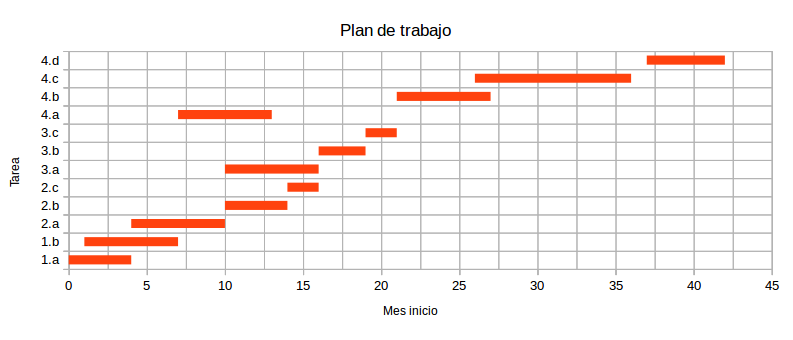
\includegraphics[width=0.95\textwidth]{./imgs/especiedegantt.png}
    \caption{Diagrama de tareas.}
    \label{fig:gantt}
  \end{center}
\end{figure*}


% Dejo esto aquí comentado para aprender cómo se hacen los diagramas de Gantt en LaTeX
%
% \definecolor{barblue}{RGB}{153,204,254}
% \definecolor{groupblue}{RGB}{51,102,254}
% \definecolor{linkred}{RGB}{165,0,33}
% \renewcommand\sfdefault{phv}
% \renewcommand\mddefault{mc}
% \renewcommand\bfdefault{bc}
% \setganttlinklabel{s-s}{EMPEZAR-PARA-EMPEZAR}
% \setganttlinklabel{f-s}{TERMINAR-PARA-EMPEZAR}
% \setganttlinklabel{f-f}{TERMINAR-PARA-TERMINAR}
% \sffamily
% 
% \begin{ganttchart}[
% canvas/.append style={fill=none, draw=black!5, line width=.75pt},
% hgrid style/.style={draw=black!5, line width=.75pt},
% vgrid={*1{draw=black!5, line width=.75pt}},
% today=7,
% today rule/.style={
% draw=black!64,
% dash pattern=on 3.5pt off 4.5pt,
% line width=1.5pt
% },
% today label font=\small\bfseries,
% title/.style={draw=none, fill=none},
% title label font=\bfseries\footnotesize,
% title label node/.append style={below=7pt},
% include title in canvas=false,
% bar label font=\mdseries\small\color{black!70},
% bar label node/.append style={left=2cm},
% bar/.append style={draw=none, fill=black!63},
% bar incomplete/.append style={fill=barblue},
% bar progress label font=\mdseries\footnotesize\color{black!70},
% group incomplete/.append style={fill=groupblue},
% group left shift=0,
% group right shift=0,
% group height=.5,
% group peaks tip position=0,
% group label node/.append style={left=.6cm},
% group progress label font=\bfseries\small,
% link/.style={-latex, line width=1.5pt, linkred},
% link label font=\scriptsize\bfseries,
% link label node/.append style={below left=-2pt and 0pt}
% ]{1}{36}
% \gantttitle[
% title label node/.append style={below left=7pt and -3pt}
% ]{MESES:\quad1}{1}
% \gantttitlelist{2,...,12}{1} \\
% \ganttgroup[progress=57]{\txt{Dispositivo}}{1}{10} \\
% \ganttbar[
% progress=75,
% name=WBS1A
% ]{\textbf{WBS 1.1} Activity A}{1}{8} \\
% \ganttbar[
% progress=67,
% name=WBS1B
% ]{\textbf{WBS 1.2} Activity B}{1}{3} \\
% \ganttbar[
% progress=50,
% name=WBS1C
% ]{\textbf{WBS 1.3} Activity C}{4}{10} \\
% \ganttbar[
% progress=0,
% name=WBS1D
% ]{\textbf{WBS 1.4} Activity D}{4}{10} \\[grid]
% \ganttgroup[progress=0]{WBS 2 Summary Element 2}{4}{10} \\
% \ganttbar[progress=0]{\textbf{WBS 2.1} Activity E}{4}{5} \\
% \ganttbar[progress=0]{\textbf{WBS 2.2} Activity F}{6}{8} \\
% \ganttbar[progress=0]{\textbf{WBS 2.3} Activity G}{9}{10}
% \ganttlink[link type=s-s]{WBS1A}{WBS1B}
% \ganttlink[link type=f-s]{WBS1B}{WBS1C}
% \ganttlink[
% link type=f-f,
% link label node/.append style=left
% ]{WBS1C}{WBS1D}
% \end{ganttchart}


\section{Medios y financiación}

La estudiante de doctorado pertenece al grupo de investigación GeNeura (TIC-024), disponiendo de financiación suficiente para la asistencia a congresos o para publicaciones en revista. Además, está prevista una contratación al menos durante un año con un proyecto relacionado con la temática de la tesis.

\part{Anexos}

\bibliographystyle{abbrv}
\bibliography{PlanTesis}

\end{document}
